\documentclass[a4paper,12pt]{jarticle}
\usepackage[dvipdfmx]{graphicx}
\usepackage{amsmath}
\usepackage{subfigure}
\usepackage{comment}
\usepackage{listings}

\setlength{\hoffset}{0cm}
\setlength{\oddsidemargin}{-3mm}
\setlength{\evensidemargin}{-3cm}
\setlength{\marginparsep}{0cm}
\setlength{\marginparwidth}{0cm}
\setlength{\textheight}{24.7cm}
\setlength{\textwidth}{17cm}
\setlength{\topmargin}{-45pt}

\renewcommand{\baselinestretch}{1.6}
\renewcommand{\floatpagefraction}{1}
\renewcommand{\topfraction}{1}
\renewcommand{\bottomfraction}{1}
\renewcommand{\textfraction}{0}
\renewcommand{\labelenumi}{(\arabic{enumi})}
%\renewcommand{\figurename}{Fig.} %図をFig.にする


%図のキャプションからコロン:を消す
\makeatletter
\long\def\@makecaption#1#2{% #1=図表番号、#2=キャプション本文
\sbox\@tempboxa{#1. #2}
\ifdim \wd\@tempboxa >\hsize
#1 #2\par 
\else
\hb@xt@\hsize{\hfil\box\@tempboxa\hfil}
\fi}
\makeatother
% 

%Listingnameの定義
\def\lstlistingname{Program}
%
\title{車両制御特論 \\
レポート2\\
}
\author{\vspace{40mm}\\
九州工業大学大学院 \hspace{0mm} 工学府\\
機械知能工学専攻\ \hspace{0mm} 知能制御工学コース \\
\vspace{5mm}\\
所属:\ 西田研究室\\
学籍番号:\ 16344217\\
提出者氏名:\ 津上 \hspace{0mm} 祐典\\\vspace{5mm}\\ }
\date{平成28年\ 8月\ 10日}

\begin{document}

%表紙
\titlepage
\maketitle
\thispagestyle{empty}

\newpage
%%%%%%%%%%%%%%%%%%%%%%%%%%%
\section{与えられたシステム}
%%%%%%%%%%%%%%%%%%%%%%%%%%%
学籍番号によって決まった制御対象は,
\begin{equation}
 \dot{x}(t) = ax^3(t) + b \cos 2t + c(x^2(t)+1)u(t) \\
\end{equation}
%
\begin{equation}
 a = 3 ,\ b = -6 , \ c = 2 
\end{equation}
%
である.また理想モデルは,
\begin{equation}
 \dot{x}_d(t) = -4x_d(t)+r_d(t)
\end{equation}
である.ここで,
\begin{equation}
 \tilde{x}(t) = x(t) - x_d(t) 
\end{equation}
おくと追従誤差方程式は,
\begin{eqnarray}
 \dot{\tilde{x}}(t) & = & \dot{x}(t) - \dot{x}_d(t) \\
 & = & ax^3(t) + b \cos 2t + c(x^2(t)+1)u(t) - \dot{x}_d(t)
\end{eqnarray}
となる.
%
%%%%%%%%%%%%%%%%%%%%%%%%%%%
\section{適応追従コントローラの設計}
%%%%%%%%%%%%%%%%%%%%%%%%%%%

%%%%%%%%%%%%%%%%%%%%%%%%%%%%%
\subsection{$a,b,c$が既知のとき}
%%%%%%%%%%%%%%%%%%%%%%%%%%%%
エネルギー関数を$V(t)=\tilde{x}^2(t)$とおく.エネルギー関数の時間微分を
解析すると,
%
\begin{eqnarray}
 \dot{V}(t) & = & 2\tilde{x}(t)\dot{\tilde{x}}(t) \\ 
  & = & 2\tilde{x}(t) \biggl[ax^3(t) + b \cos 2t+c\bigl\{x^2(t)+1 \bigr\}u(t)-\dot{x}_d(t)\biggr] 
\end{eqnarray}
%
となる.ここで入力$u(t)$を
\begin{equation}
 u(t) = -\frac{ax^3(t)}{c(x^2(t)+1)} -\frac{b \cos 2t}{c(x^2(t)+1)}
  +\frac{\dot{x}_d(t)}{c(x^2(t)+1)} - \delta \tilde{x}(t) \ \ \ \ (\delta > 0)
\end{equation}
%
とすれば,
%
\begin{equation}
 \dot{V}(t) = -2\delta c (x^2(t)+1)\tilde{x}^2(t) < 0 \ \ \ \ \ \ for \ any \ \tilde{x}(t)\neq 0
\end{equation}
となり,システムを漸近安定化することが出来る.
%%%%%%%%%%%%%%%%%%%%%%%%%%%%%
\subsection{$a,b,c$が未知のとき}
%%%%%%%%%%%%%%%%%%%%%%%%%%%%
次に,$a,b,c$が未知な場合を考える.入力$u(t)$を
\begin{eqnarray}
 u(t)& = & -\frac{\hat{a}}{\hat{c}}\frac{x^3(t)}{x^2(t)+1} -\frac{\hat{b}}{\hat{c}}\frac{\cos 2t}{x^2(t)+1}
  +\frac{1}{\hat{c}}\frac{\dot{x}_d(t)}{x^2(t)+1} - \delta \tilde{x}(t) \\
  & = & -\hat{\alpha}\frac{x^3(t)}{x^2(t)+1} +\hat{\beta}\frac{\cos 2t}{x^2(t)+1}
  +\hat{\gamma}\frac{\dot{x}_d(t)}{x^2(t)+1} - \delta \tilde{x}(t)
\end{eqnarray}
%
とすると,誤差追従方程式は,
%
\begin{eqnarray}
 \dot{\tilde{x}}(t) &=& ax^3(t) + b \cos 2t - \dot{x}_d(t) -c\hat{\alpha}x^3(t) -c\hat{\beta}\cos 2t
  +c\hat{\gamma}\dot{x}_d(t) - c\delta \bigl\{x^2(t) + 1 \bigr\} \tilde{x}(t)\\
  &=&c\tilde{\alpha}x^3(t) +c\tilde{\beta}\cos 2t
  -c\tilde{\gamma}\dot{x}_d(t) - c\delta \bigl\{x^2(t)+1 \bigr\}\tilde{x}(t)
\end{eqnarray}
となる.エネルギー関数を
\begin{equation}
 V(t) = \tilde{x}^2(t) + \eta^{-1}_{\alpha}c\tilde{\alpha}^2+\eta^{-1}_{\beta}c\tilde{\beta}^2+\eta^{-1}_{\gamma}c\tilde{\gamma}^2
\end{equation}
とおく.ただし,
$\eta_{\alpha},\eta_{\beta},\eta_{\gamma}$は推定ゲインで
ある.次に,エネルギー関数の時間微分を解析すると,
%
\begin{equation}
\dot{V}(t) =  2\tilde{x}(t)\dot{\tilde{x}}(t) +
 2\eta^{-1}_{\alpha}c\tilde{\alpha}\dot{\tilde{\alpha}}
 +2\eta^{-1}_{\beta}c\tilde{\beta}\dot{\tilde{\beta}} +
 2\eta^{-1}_{\gamma}c\tilde{\gamma}\dot{\tilde{\gamma}}
\end{equation}
%
より
\begin{eqnarray}
   \dot{V}(t)&=& 2\tilde{x}(t)\bigl[ c\tilde{\alpha}x^3(t) +c\tilde{\beta}\cos 2t
  -c\tilde{\gamma}\dot{x}_d(t) - c\delta \bigl\{x^2(t)+1\bigr\}
 \tilde{x}(t)\bigr]\\ 
& & + 2\eta^{-1}_{\alpha}c\tilde{\alpha}\dot{\tilde{\alpha}}
 +2\eta^{-1}_{\beta}c\tilde{\beta}\dot{\tilde{\beta}} +
  2\eta^{-1}_{\gamma}c\tilde{\gamma}\dot{\tilde{\gamma}} 
\end{eqnarray}
%
となる.ここで,
\begin{eqnarray}
\dot{\tilde{\alpha}}&=&-\dot{\hat{\alpha}}=-\eta_{\alpha}\tilde{x}(t)x^3(t) \\
\dot{\tilde{\beta}}&=&-\dot{\hat{\beta}}=-\eta_{\beta}\cos 2t \tilde{x}(t) \\
\dot{\tilde{\gamma}}&=&-\dot{\hat{\gamma}}=\eta_{\gamma}\tilde{x}(t)\dot{x}_d(t)   
\end{eqnarray}
とすれば,
%
\begin{equation}
\dot{V}(t) = -2\delta c (x^2(t)+1)\tilde{x}^2(t) \leq 0 \ \ \ \ \ \ for \ any \ \ \begin{pmatrix}
\tilde{x}(t)\\ \tilde{\alpha}\\ \tilde{\beta}\\ \tilde{\gamma}\\
\end{pmatrix}
\neq
\begin{pmatrix}
0\\ 0\\ 0\\ 0\\ 
\end{pmatrix}								
\end{equation}
%
となり,システムを安定化出来る.

以上より,以下の適応追従コントローラを得る.

\begin{eqnarray}
  u(t)&=& -\hat{\alpha}\frac{x^3(t)}{x^2(t)+1} +\hat{\beta}\frac{\cos 2t}{x^2(t)+1}
  +\hat{\gamma}\frac{\dot{x}_d(t)}{x^2(t)+1} - \delta \tilde{x}(t) \\
  \dot{\hat{\theta}}(t)
  &=&
  \begin{pmatrix}
	 \dot{\hat{\alpha}}\\ \dot{\hat{\beta}}\\ \dot{\hat{\gamma}}\\
  \end{pmatrix}
  =
  \begin{pmatrix}
   \eta_{\alpha}\tilde{x}(t)x^3(t)\\
   \eta_{\beta}\cos 2t \tilde{x}(t)\\
   -\eta_{\gamma}\tilde{x}(t)\dot{x}_d(t)\\
  \end{pmatrix}
\end{eqnarray}

%%%%%%%%%%%%%%%%%%%%%%%%%%%%%
\section{シミュレーション}
%%%%%%%%%%%%%%%%%%%%%%%%%%%%
simulinkで構成したモデルを示す.
%
\begin{figure}[htb]
    \begin{center}
       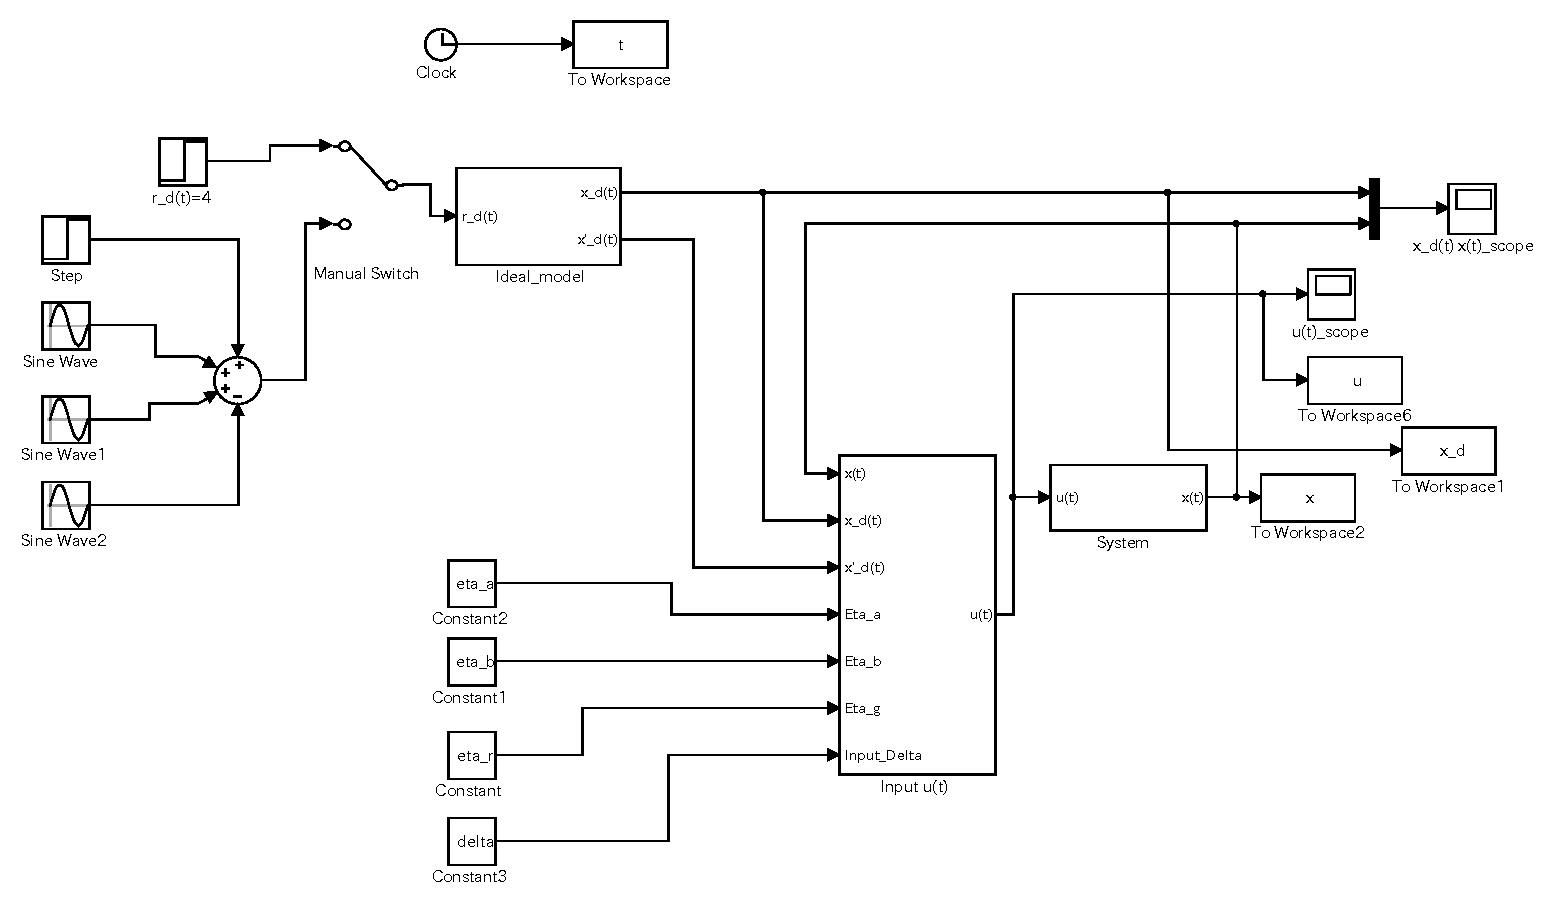
\includegraphics[width=170mm]{fig/zentai.eps}
        \caption{構成したモデル}
        \label{fig:zentai}
    \end{center}
 \end{figure}
%
%
\begin{figure}[htb]
    \begin{center}
       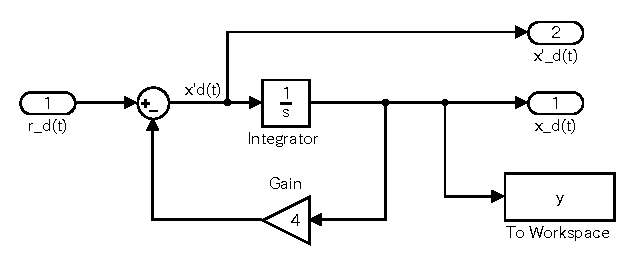
\includegraphics[width=100mm]{fig/ideal.eps}
        \caption{理想モデル}
        \label{fig:ideal}
    \end{center}
 \end{figure}
 %
 %
\begin{figure}[htb]
    \begin{center}
       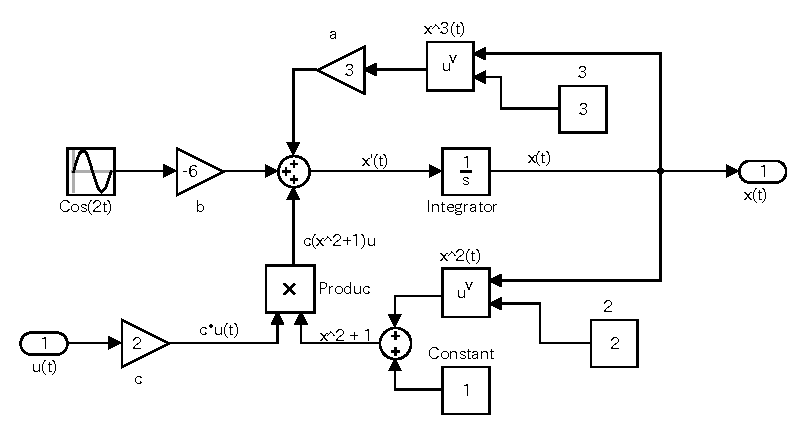
\includegraphics[width=100mm]{fig/System.eps}
        \caption{制御対象}
        \label{fig:System}
    \end{center}
 \end{figure}
%
%
\begin{figure}[htb]
    \begin{center}
       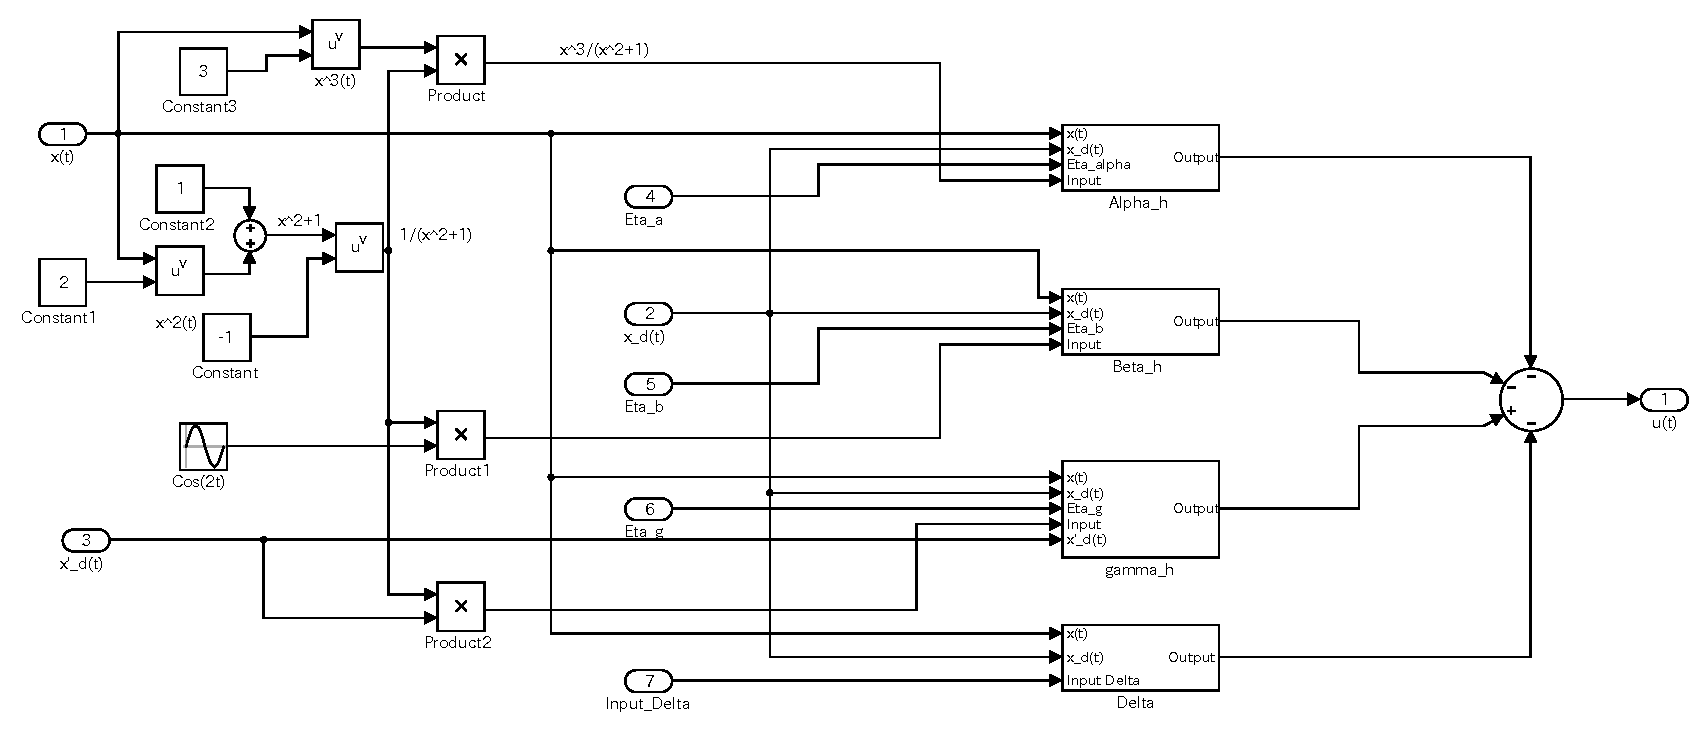
\includegraphics[width=100mm]{fig/input.eps}
        \caption{入力}
        \label{fig:input}
    \end{center}
 \end{figure}
 %
 %
\begin{figure}[htb]
    \begin{center}
       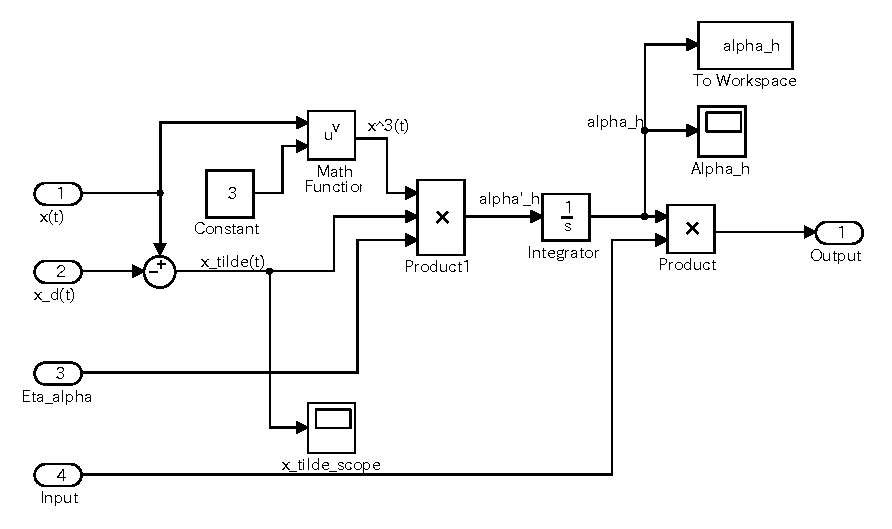
\includegraphics[width=100mm]{fig/alpha.eps}
        \caption{$\alpha$}
        \label{fig:alpha}
    \end{center}
 \end{figure}
 %
%
\begin{figure}[htb]
    \begin{center}
       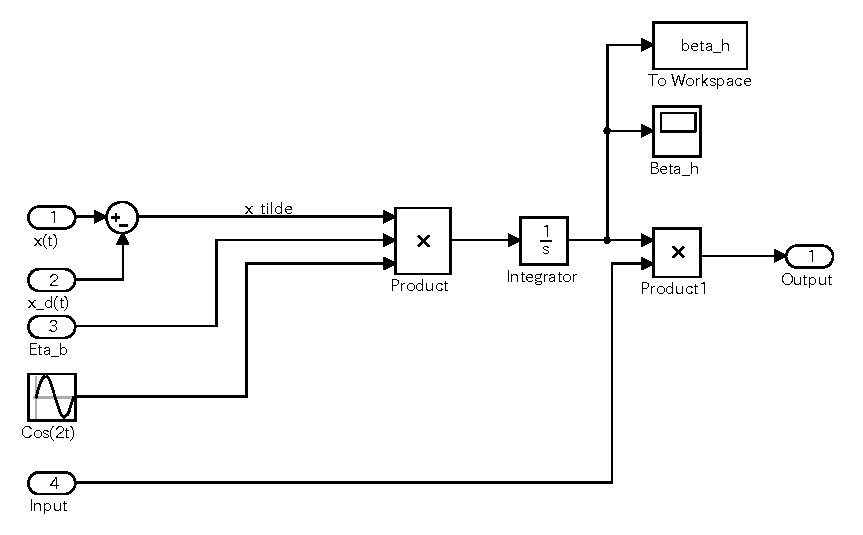
\includegraphics[width=100mm]{fig/beta.eps}
        \caption{$\beta$}
        \label{fig:beta}
    \end{center}
 \end{figure}
%
%
\begin{figure}[htb]
    \begin{center}
       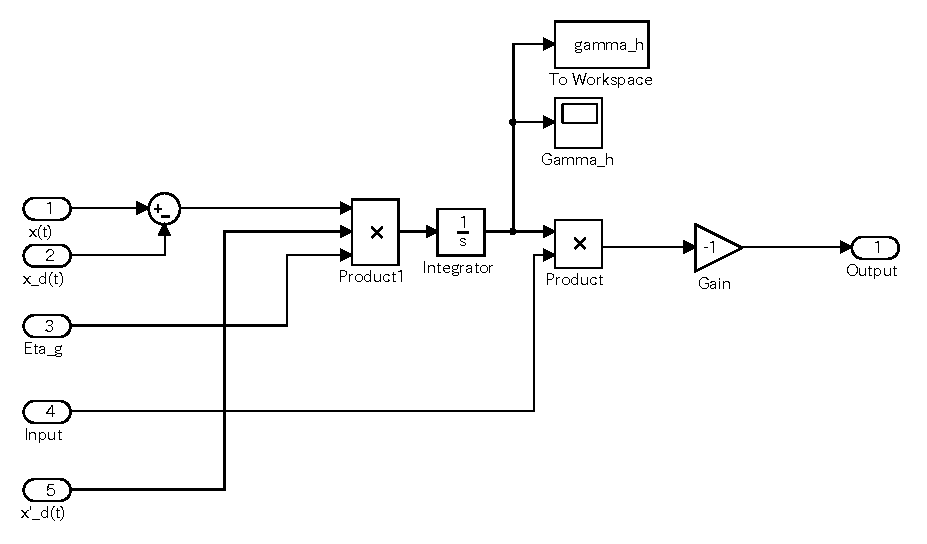
\includegraphics[width=100mm]{fig/gamma.eps}
        \caption{$\gamma$}
        \label{fig:gamma}
    \end{center}
 \end{figure}
%
%
\begin{figure}[htb]
    \begin{center}
       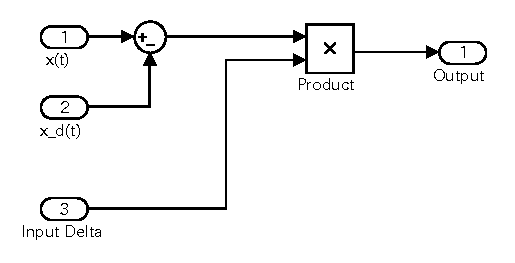
\includegraphics[width=100mm]{fig/delta.eps}
        \caption{$\delta$}
        \label{fig:delta}
    \end{center}
 \end{figure}
%


 
%%%%%%%%%%%%%%%%%%%%%%%%%%%%%
\subsection{$r_d(t)=4$の場合}
%%%%%%%%%%%%%%%%%%%%%%%%%%%%


%%%%%%%%%%%%%%%%%%%%%%%%%%%%%
\subsection{$r_d(t)=4+0.5\sin 0.5t + \cos 3t - 2\sin 5t$の場合}
%%%%%%%%%%%%%%%%%%%%%%%%%%%%


%%%%%%%%%%%%%%%%%%%%%%%%%%%%%
\section{考察}
%%%%%%%%%%%%%%%%%%%%%%%%%%%%

\begin{thebibliography}{99}
\addcontentsline{toc}{section}{参考文献}

 \bibitem{jamming} 大屋勝敬:"車両制御特論MATLAB+Simulinkの利用法"
\end{thebibliography}

\end{document}
